\chapter{Implementasi dan Simulasi}
\label{ch:implementasi}

\section{Lingkungan dan Struktur Program}
\algname{} diimplementasikan dalam Python 3.13 tanpa pustaka kriptografi eksternal. Fungsi enkripsi dan dekripsi hanya memakai pustaka standar (\code{secrets} untuk \textit{nonce}, \code{hashlib} untuk SHA-256 pada penjadwalan kunci, dan \code{base64} untuk pengodean keluaran). Pustaka \code{numpy} dan \code{matplotlib} hanya dipakai oleh modul analisis. Struktur modulnya ditunjukkan pada \cref{tab:modul}.

\begin{table}[H]
    \centering
    \caption{Struktur modul pada paket \code{src}}
    \label{tab:modul}
    \small
    \begin{tabularx}{\textwidth}{l Y}
        \toprule
        \textbf{Modul} & \textbf{Tanggung jawab} \\
        \midrule
        \code{encrypt.py}, \code{decrypt.py} & Antarmuka utama \code{encrypt()} dan \code{decrypt()} \\
        \code{keygen.py} & Validasi dan \textit{hashing} kunci, pembangkitan \textit{nonce}, pengisian spiral, paritas, \textit{whitening}, dan penurunan 18 \textit{round key} \\
        \code{automaton.py} & Game of Life bit-paralel pada grid toroidal (pohon penjumlah, aturan B3/S23) \\
        \code{feistel.py} & Jaringan Feistel 18 ronde, pemilihan fungsi ronde, dan $f_{\text{GoL}}$ \\
        \code{spn.py} & $f_{\text{SPN}}$: Kotak-S, \code{ShiftRows}, \code{MixColumns}, penjumlahan modular, rotasi bergantung data \\
        \code{modes.py} & Mode operasi ECB, CBC, CFB, OFB, dan CTR \\
        \code{padding.py} & \textit{Padding} PKCS\#7 dan validasinya \\
        \code{types.py} & Tipe data \code{Grid} (setiap baris disimpan sebagai \textit{bitmask} bilangan bulat) \\
        \code{analysis.py} & Uji \textit{avalanche}, entropi, dan histogram \\
        \bottomrule
    \end{tabularx}
\end{table}

\section{Antarmuka Program}
\algname{} disediakan sebagai pustaka Python dengan dua fungsi utama:
\begin{itemize}
    \item \code{encrypt(data, key, mode="CBC") -> bytes}: menerima \textit{plaintext} berupa \code{str}, \code{bytes}, atau \code{bytearray} (teks maupun isi berkas biner) dan mengembalikan Base64 dari $N \Vert C$;
    \item \code{decrypt(data, key, mode="CBC") -> bytes}: menerima keluaran \code{encrypt()} dan mengembalikan \textit{plaintext} asli dalam bentuk \code{bytes}.
\end{itemize}
Contoh pemakaian untuk teks dan berkas biner ditunjukkan pada \cref{lst:contoh}.

\noindent\begin{minipage}{\linewidth}
\begin{lstlisting}[language=Python, caption={Contoh pemakaian \code{encrypt()} dan \code{decrypt()}}, label={lst:contoh}]
from src.encrypt import encrypt
from src.decrypt import decrypt

key = "kunci-rahasia-minimal-32-byte!!!"           # 32 byte
ct = encrypt("Halo, dunia!", key, mode="CTR")      # bytes Base64
assert decrypt(ct, key, mode="CTR") == b"Halo, dunia!"

with open("test/berkas/image.jpg", "rb") as f:     # berkas biner
    data = f.read()
ct = encrypt(data, key, mode="OFB")
assert decrypt(ct, key, mode="OFB") == data
\end{lstlisting}
\end{minipage}

Pustaka ini didistribusikan melalui halaman \textit{Releases} di GitHub. Setiap kali ada perubahan di \textit{branch} \code{main}, GitHub Actions otomatis membuat rilis baru berisi arsip \code{pregnant\_sister-vX.Y.Z.zip} (dan \code{.tar.gz}). Arsip ini memuat seluruh isi repositori: kode pustaka (\code{src}), \code{requirements.txt}, \textit{test} beserta berkas ujinya, laporan, dan dokumentasi API. Pengguna cukup mengekstrak arsip, menjalankan \code{pip install -r requirements.txt}, lalu mengimpor \code{src.encrypt} dan \code{src.decrypt} atau menjalankan skrip pengujian dari akar arsip.

Dokumentasi API lengkap dipublikasikan di \url{https://cola1000.github.io/Pregnant_Sister/} (\cref{fig:api}). Dokumentasi ini memuat cara instalasi dari rilis, parameter dan tipe data kedua fungsi, format \textit{ciphertext}, mode operasi, contoh penggunaan, penanganan galat, serta catatan keamanan.

\begin{figure}[H]
    \centering
    \fbox{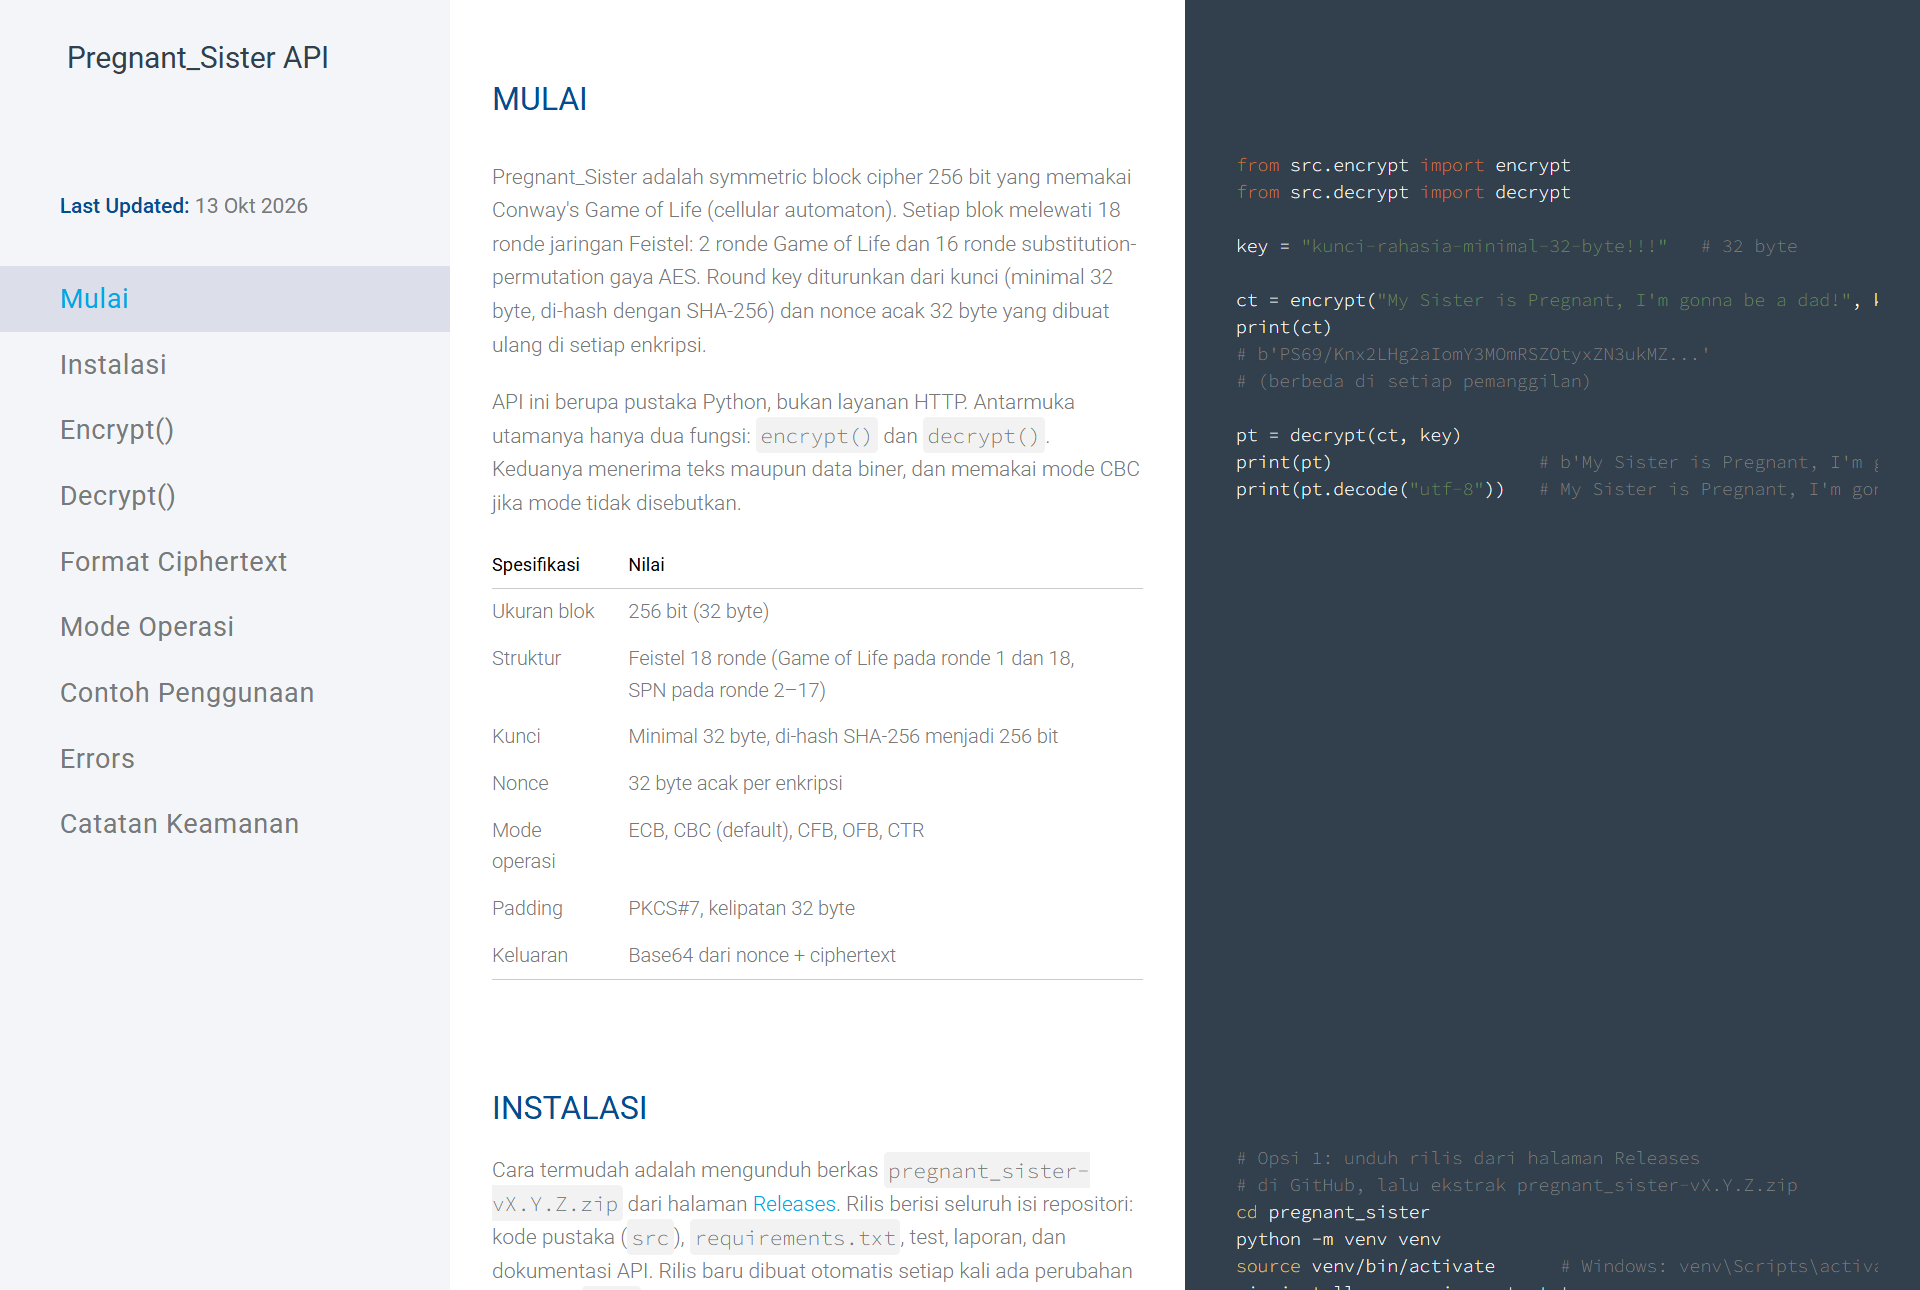
\includegraphics[width=0.92\textwidth]{api_docs.png}}
    \caption{Halaman dokumentasi API \algname}
    \label{fig:api}
\end{figure}

Selain pustaka, repositori menyediakan skrip pengujian yang dijalankan dari direktori akar (\cref{lst:skrip}).

\noindent\begin{minipage}{\linewidth}
\begin{lstlisting}[language=bash, caption={Skrip pengujian yang tersedia}, label={lst:skrip}]
python -m test.test_text        # analisis berkas teks (CBC)
python -m test.test_image       # analisis berkas gambar (CBC)
python -m test.test_video       # analisis berkas video (CBC)
python -m test.test_encrypt     # round-trip lima mode untuk semua berkas
python -m test.test_security    # evaluasi keamanan (Bab 5)
python -m test.test_keygen      # unit test penjadwalan kunci
python -m test.test_automaton   # unit test Game of Life
\end{lstlisting}
\end{minipage}

\section{Skenario Pengujian}
Pengujian dilakukan pada tiga berkas di \code{test/berkas} (\cref{tab:berkas}) dengan kunci 35 byte \code{"000\ldots0"} (35 karakter \code{'0'}). Kunci ini sengaja dipilih berpola agar terlihat bahwa \textit{ciphertext} tetap tampak acak walaupun kuncinya lemah secara visual. Berkas teks dan citra diuji pada kelima mode, sedangkan berkas video diuji pada mode CBC. Untuk setiap pengujian, kami mencatat ukuran \textit{ciphertext}, waktu enkripsi dan dekripsi, serta \textit{hash} SHA-256 dari \textit{plaintext} asli dan hasil dekripsi. Seluruh pengujian dijalankan pada mesin pengembang (Windows 11, Python 3.13.7).

\begin{table}[H]
    \centering
    \caption{Berkas uji}
    \label{tab:berkas}
    \begin{tabular}{l l r}
        \toprule
        \textbf{Berkas} & \textbf{Jenis} & \textbf{Ukuran (byte)} \\
        \midrule
        \code{glasses.txt} & teks ASCII berbahasa Inggris & 1.032 \\
        \code{image.jpg} & biner (citra JPEG) & 833.290 \\
        \code{video.mp4} & biner (video MP4) & 39.228.657 \\
        \bottomrule
    \end{tabular}
\end{table}

\section{Hasil Enkripsi dan Dekripsi}

\subsection{Berkas Teks}
\Cref{tab:hasil-teks} menunjukkan bahwa kelima mode mengembalikan berkas teks secara utuh. \textit{Ciphertext} mentah berukuran 1.088 byte, yaitu 32 byte \textit{nonce} ditambah 1.056 byte data (1.032 byte \textit{plaintext} ditambah 24 byte \textit{padding}). Walaupun \textit{plaintext} dan kuncinya sama, awalan \textit{ciphertext} berbeda pada setiap mode dan setiap eksekusi karena \textit{nonce} dibangkitkan secara acak.

\begin{table}[H]
    \centering
    \caption{Hasil enkripsi--dekripsi \code{glasses.txt} (SHA-256 \textit{plaintext} = \code{76d3bcab876abc41\ldots})}
    \label{tab:hasil-teks}
    \small\setlength{\tabcolsep}{4pt}
    \begin{tabular}{l r r r l c}
        \toprule
        \textbf{Mode} & \textbf{Mentah (B)} & \textbf{Base64 (B)} & \textbf{Enk + Dek (s)} & \textbf{Awalan Base64} & \textbf{SHA-256 sama} \\
        \midrule
        ECB & 1.088 & 1.452 & 0,02 + 0,02 & \code{FausVPMQ6FdvselD\ldots} & \checkmark \\
        CBC & 1.088 & 1.452 & 0,02 + 0,02 & \code{TMbd8jBi5LTpdZ4/\ldots} & \checkmark \\
        CFB & 1.088 & 1.452 & 0,02 + 0,02 & \code{FfINU8zWIv2+NQvq\ldots} & \checkmark \\
        OFB & 1.088 & 1.452 & 0,02 + 0,02 & \code{zpFhCn8xRThkoAne\ldots} & \checkmark \\
        CTR & 1.088 & 1.452 & 0,03 + 0,03 & \code{s4IBPE0rgSBj4nmc\ldots} & \checkmark \\
        \bottomrule
    \end{tabular}
\end{table}

\subsection{Berkas Biner}
\Cref{tab:hasil-biner} menunjukkan hasil untuk berkas citra JPEG. Kelima mode kembali mengembalikan berkas secara utuh, dan berkas hasil dekripsi dapat dibuka kembali sebagai gambar yang identik dengan aslinya. Waktu proses sekitar 12--14 detik per arah, yang setara dengan laju sekitar 60--70 KB/s. Laju ini wajar untuk implementasi Python murni yang menjalankan 18 ronde Feistel per blok.

\begin{table}[H]
    \centering
    \caption{Hasil enkripsi--dekripsi \code{image.jpg} (SHA-256 \textit{plaintext} = \code{5a92b5ae1f92711d\ldots})}
    \label{tab:hasil-biner}
    \small\setlength{\tabcolsep}{4pt}
    \begin{tabular}{l r r r l c}
        \toprule
        \textbf{Mode} & \textbf{Mentah (B)} & \textbf{Base64 (B)} & \textbf{Enk + Dek (s)} & \textbf{Awalan Base64} & \textbf{SHA-256 sama} \\
        \midrule
        ECB & 833.344 & 1.111.128 & 12,38 + 14,23 & \code{omJYfWOjziOuq/N2\ldots} & \checkmark \\
        CBC & 833.344 & 1.111.128 & 11,83 + 12,07 & \code{OZKtQ6Sq7KdFkgfE\ldots} & \checkmark \\
        CFB & 833.344 & 1.111.128 & 11,99 + 11,81 & \code{ZrkGsc34edw8uSqx\ldots} & \checkmark \\
        OFB & 833.344 & 1.111.128 & 12,04 + 11,70 & \code{d8268e8ICcqGvbgH\ldots} & \checkmark \\
        CTR & 833.344 & 1.111.128 & 11,65 + 11,96 & \code{pW908tgQo8GVnHXq\ldots} & \checkmark \\
        \bottomrule
    \end{tabular}
\end{table}

Berkas video 39 MB hanya diuji dengan mode CBC, karena setiap arah membutuhkan sekitar 10 menit (\cref{tab:hasil-video}). Kebenaran kelima mode pada data biner sudah ditunjukkan oleh berkas citra. Skrip \code{test.test\_encrypt} tetap dapat dipakai untuk menguji video pada kelima mode, dengan waktu total sekitar 1,5 jam.

\begin{table}[H]
    \centering
    \caption{Hasil enkripsi--dekripsi \code{video.mp4} (SHA-256 \textit{plaintext} = \code{f8564e7de424642c\ldots})}
    \label{tab:hasil-video}
    \small\setlength{\tabcolsep}{4pt}
    \begin{tabular}{l r r r l c}
        \toprule
        \textbf{Mode} & \textbf{Mentah (B)} & \textbf{Base64 (B)} & \textbf{Enk + Dek (s)} & \textbf{Awalan Base64} & \textbf{SHA-256 sama} \\
        \midrule
        CBC & 39.228.704 & 52.304.940 & 594,45 + 563,29 & \code{3Li8Ac7JD1iAs7lM\ldots} & \checkmark \\
        \bottomrule
    \end{tabular}
\end{table}

\subsection{Enkripsi Probabilistik}
Mengenkripsi \textit{plaintext} \code{"Halo, dunia!"} dua kali dengan kunci dan mode yang sama menghasilkan dua \textit{ciphertext} yang sama sekali berbeda:
\begin{center}
    \code{sBYT/+P7ag6EmtcTZWO8guwS4HL5BWw8fa9oNjwaFlEZ\ldots} \\
    \code{oqGOzWvLxJ8o32eP/q0z4RkpiObsWrgvPF7z4Klit3SQ\ldots}
\end{center}
Kedua \textit{ciphertext} tetap terdekripsi menjadi \textit{plaintext} yang sama. Sifat ini mencegah penyerang mengetahui apakah dua pesan memiliki isi yang sama.

\section{Analisis Penanganan Padding}
\label{sec:analisis-padding}
\Cref{tab:padding} menunjukkan perilaku \textit{padding} pada panjang \textit{plaintext} di sekitar batas blok. Untuk setiap panjang, dilakukan \textit{round-trip} pada kelima mode, dan semuanya berhasil.

\begin{table}[H]
    \centering
    \caption{Perilaku \textit{padding} PKCS\#7 (blok 32 byte) pada berbagai panjang \textit{plaintext}}
    \label{tab:padding}
    \small
    \begin{tabular}{r r r l r c}
        \toprule
        \textbf{$|P|$ (B)} & \textbf{$p$} & \textbf{\shortstack{Setelah\\\textit{padding} (B)}} & \textbf{\shortstack{Byte terakhir\\(heks)}} & \textbf{\shortstack{Mentah +\\\textit{nonce} (B)}} & \textbf{\shortstack{\textit{Round-trip}\\5 mode}} \\
        \midrule
        0   & 32 & 32  & \code{20 20 20 \ldots\ 20} & 64  & \checkmark \\
        1   & 31 & 32  & \code{1f 1f 1f \ldots\ 1f} & 64  & \checkmark \\
        15  & 17 & 32  & \code{11 11 11 \ldots\ 11} & 64  & \checkmark \\
        31  & 1  & 32  & \code{01}                  & 64  & \checkmark \\
        32  & 32 & 64  & \code{20 20 20 \ldots\ 20} & 96  & \checkmark \\
        33  & 31 & 64  & \code{1f 1f 1f \ldots\ 1f} & 96  & \checkmark \\
        63  & 1  & 64  & \code{01}                  & 96  & \checkmark \\
        64  & 32 & 96  & \code{20 20 20 \ldots\ 20} & 128 & \checkmark \\
        100 & 28 & 128 & \code{1c 1c 1c \ldots\ 1c} & 160 & \checkmark \\
        \bottomrule
    \end{tabular}
\end{table}

Ada tiga hal penting dari hasil ini:
\begin{enumerate}
    \item \textbf{\textit{Padding} selalu ditambahkan.} \textit{Plaintext} kosong dan \textit{plaintext} yang panjangnya kelipatan 32 (0, 32, 64 byte) mendapat satu blok \textit{padding} penuh bernilai \code{0x20}. Tanpa aturan ini, \textit{plaintext} yang kebetulan berakhir dengan byte \code{0x01} tidak dapat dibedakan dari \textit{padding}.
    \item \textbf{\textit{Padding} juga dipakai pada mode aliran.} CFB, OFB, dan CTR sebenarnya tidak memerlukan \textit{padding}, tetapi rancangan kami tetap menerapkannya agar format \textit{ciphertext} seragam untuk semua mode. Konsekuensinya, \textit{ciphertext} selalu 1--32 byte lebih panjang dari \textit{plaintext}.
    \item \textbf{\textit{Padding} divalidasi saat dekripsi.} Fungsi \code{unpad} menolak nilai $p$ di luar rentang 1--32 dan $p$ byte terakhir yang tidak seragam. Validasi ini juga berfungsi sebagai pendeteksi kesalahan sederhana (\cref{sec:integritas}).
\end{enumerate}

\section{Verifikasi Integritas Data}
\label{sec:integritas}

\subsection{Kecocokan Hash}
Integritas hasil dekripsi diverifikasi dengan membandingkan \textit{hash} SHA-256 berkas asli dan berkas hasil dekripsi. Pada \cref{tab:hasil-teks,tab:hasil-biner,tab:hasil-video}, kesebelas pasangan berkas dan mode menghasilkan \textit{hash} yang identik, sehingga hasil dekripsi sama persis bit demi bit dengan berkas asli. \textit{Hash} lengkapnya dicantumkan pada \cref{app:hash}. Pengujian \code{test\_security} juga menjalankan \textit{round-trip} untuk panjang 0, 1, 31, 32, 33, dan 100 byte dengan kunci acak sepanjang 32--71 byte pada kelima mode, dan tidak ada satu pun kegagalan.

\subsection{Deteksi Kunci atau Mode yang Salah}
Validasi \textit{padding} memberikan deteksi kesalahan secara tidak langsung. Jika kunci salah, blok terakhir hasil dekripsi praktis acak, sehingga peluang \textit{padding}-nya kebetulan valid sekitar $\sum_{p=1}^{32} 2^{-8p} \approx 1/255$. Hasil eksperimen pada \cref{tab:deteksi} sesuai dengan perkiraan tersebut.

\begin{table}[H]
    \centering
    \caption{Deteksi dekripsi dengan kunci atau mode yang salah (400 percobaan per skenario)}
    \label{tab:deteksi}
    \begin{tabular}{l r r}
        \toprule
        \textbf{Skenario} & \textbf{Terdeteksi (\code{ValueError})} & \textbf{Lolos tanpa galat} \\
        \midrule
        Kunci salah, mode CBC & 399 & 1 \\
        Kunci salah, mode CTR & 397 & 3 \\
        Enkripsi CBC, dekripsi CTR & 399 & 1 \\
        \bottomrule
    \end{tabular}
\end{table}

\subsection{Deteksi Perubahan Ciphertext}
Untuk menguji apakah perubahan pada \textit{ciphertext} terdeteksi, kami membalik satu bit pada blok kedua \textit{ciphertext} sebuah pesan empat blok, lalu menghitung jumlah bit yang berubah pada setiap blok hasil dekripsi (\cref{tab:propagasi}). Kami juga membalik satu bit acak pada blok terakhir sebanyak 300 kali per mode.

\begin{table}[H]
    \centering
    \caption{Propagasi galat akibat pembalikan 1 bit pada blok \textit{ciphertext} $C_2$ (jumlah bit berubah dari 256 bit per blok \textit{plaintext})}
    \label{tab:propagasi}
    \begin{tabular}{l c c c c c c r}
        \toprule
        \textbf{Mode} & $P_1$ & $P_2$ & $P_3$ & $P_4$ & $P_5$ (\textit{pad}) & \textbf{Terdeteksi?} & \textbf{Ubah blok terakhir terdeteksi} \\
        \midrule
        ECB & 0 & 120 & 0 & 0 & 0 & tidak & 299/300 \\
        CBC & 0 & 130 & 1 & 0 & 0 & tidak & 298/300 \\
        CFB & 0 & 1 & 126 & 0 & 0 & tidak & 133/300 \\
        OFB & 0 & 1 & 0 & 0 & 0 & tidak & 125/300 \\
        CTR & 0 & 1 & 0 & 0 & 0 & tidak & 131/300 \\
        \bottomrule
    \end{tabular}
\end{table}

Hasil ini sesuai dengan teori mode operasi. Pada ECB dan CBC, blok yang diubah terdekripsi menjadi data acak, dan pada CBC satu bit yang sama juga ikut terbalik di blok berikutnya. Pada CFB terjadi kebalikannya: bit yang sama terbalik di blok tersebut, lalu blok berikutnya rusak. Pada OFB dan CTR, hanya bit yang sama di \textit{plaintext} yang terbalik. \textbf{Tidak satu pun perubahan di tengah pesan terdeteksi}, karena blok \textit{padding} tidak tersentuh.

Perubahan pada blok terakhir terdeteksi hampir selalu pada ECB/CBC (seluruh blok terakhir menjadi acak sehingga \textit{padding} rusak). Pada mode aliran, perubahan hanya terdeteksi jika bit yang dibalik jatuh di area \textit{padding} (14 dari 32 byte pada pesan ini, sekitar 44\%). Kesimpulannya, \textbf{validasi \textit{padding} bukan mekanisme integritas}. \algname{} memberikan kerahasiaan, tetapi tidak memberikan autentikasi pesan. Implikasi keamanannya dibahas pada \cref{sec:integritas-keamanan}.
